\section{Spin-Boson First Example}
\label{sec:spin_boson_example}

\paragraph{Role in paper.}
This section is an instantiation of the general framework, not the conceptual centre of the
manuscript. The general theory is already complete before this example.
The spin-boson model is used because it is the canonical finite-dimensional benchmark where
mean-force weak/ultrastrong structure is explicit
\cite{leggettDynamicsDissipativeTwostate1987,cresserWeakUltrastrongCoupling2021a}.

\subsection{Specialisation from the general framework}

\paragraph{Model and closed parameters.}
\begin{align}
  H_Q &= \frac{\omega_q}{2}\sigma_z, \\
  H_X &= \sum_k \omega_k b_k^\dagger b_k, \\
  f(\theta) &= \cos\theta\,\sigma_z - \sin\theta\,\sigma_x, \\
  B &= \sum_k c_k(b_k+b_k^\dagger), \\
  H_{\mathrm{int}} &= g\,f(\theta)\otimes B, \\
  H_{\mathrm{tot}} &= H_Q + H_X + H_{\mathrm{int}}.
\end{align}

Using Definition~\ref{def:influence_operator}, the reduced equilibrium operator is partitioned as
\begin{equation}
  \frac{\bar{\rho}_Q(\beta)}{Z_X(\beta)}
  = e^{-\beta H_Q/2}\,e^S\,e^{-\beta H_Q/2},
\end{equation}
where \(S\equiv S_\beta\) is the qubit influence generator.

For a Gaussian bath, closure compresses bath dependence into \(\Sigma_z(\beta,g)\) and
\(\Sigma_\perp(\beta,g)\)
\cite{cresserWeakUltrastrongCoupling2021a,cerisolaQuantumClassicalCorrespondence2024,mccaulMeanForceHamiltoniansInfluence2026}. With \(c=\cos\theta\), \(s=\sin\theta\), define
\begin{align}
  \chi &:= s\sqrt{c^2\Sigma_\perp^2+s^2\Sigma_z^2}, \\
  \gamma(\chi) &:= \frac{\tanh\chi}{\chi}, \\
  \Theta &:= \operatorname{arctanh}\!\big(\gamma(\chi)s^2\Sigma_z\big)-\frac{\beta\omega_q}{2}, \\
  m_z &:= \tanh\Theta,
  \qquad
  r := |\tanh\chi|, \\
  \tan\eta &:= -\cot\theta \,\frac{\Sigma_\perp}{\Sigma_z}.
\end{align}
Hence radial data \((r,\mathcal{P})\) are controlled by \(\chi\), while directional data are
controlled by \((\eta,\Theta)\).

\paragraph{Single-channel scaling.}
With \(K(u)=g^2K_0(u)\), one has
\begin{equation}
  \Sigma_z(\beta,g)=g^2\Sigma_z^{(0)}(\beta),
  \qquad
  \Sigma_\perp(\beta,g)=g^2\Sigma_\perp^{(0)}(\beta),
\end{equation}
so
\begin{align}
  \chi(\beta,g,\theta) &= g^2\chi_0(\beta,\theta), \\
  \chi_0(\beta,\theta) &:= s\sqrt{c^2(\Sigma_\perp^{(0)})^2+s^2(\Sigma_z^{(0)})^2},
\end{align}
and
\begin{equation}
  g_\star(\beta,\theta)=\chi_0(\beta,\theta)^{-1/2},
  \qquad
  g^\vee=\frac{g_\star^2}{g}.
\end{equation}

\subsection{\texorpdfstring{Easy \(g \to \infty\) route via the influence operator}{Easy g->infty route via the influence operator}}

\paragraph{Why this limit is easy.}
Use the symmetrized influence generator
\begin{equation}
  S = \Delta_0\I + \Delta_z \sigma_z + \Delta_\perp
  (\sigma_x\cos\phi_f + \sigma_y\sin\phi_f).
\end{equation}
Let \(M:=S-\Delta_0\I\), \(M^2=\chi^2\I\). Then exactly
\begin{equation}
  e^S = e^{\Delta_0}\cosh\chi\left(\I+\gamma M\right),
  \qquad \gamma=\frac{\tanh\chi}{\chi},
\end{equation}
and
\begin{equation}
  \rho_\Delta=\frac{e^S}{\Tr e^S}.
\end{equation}
No additional resummation is required: one evaluates closed functions of \(\chi\), \(\Delta_z\),
\(\Delta_\perp\), then takes limits.

\begin{proposition}[Easy-limit statement]
\label{prop:easy_limit_spin_boson}
At fixed \((\beta,\theta)\), the \(g\to\infty\) asymptotic in the spin-boson closure is directly
controlled by the influence-state representation \(\rho_\Delta=e^S/\Tr e^S\). In particular, the
radial part saturates as \(r\to 1\) through \(\tanh\chi\), while orientation is obtained from finite
ratios encoded in \((\Delta_z,\Delta_\perp)\) through \(\gamma M\).
\end{proposition}
\begin{proof}
Under single-channel scaling, \(\chi=g^2\chi_0\to\infty\) for fixed \((\beta,\theta)\) with
\(\chi_0>0\). Hence \(\tanh\chi\to 1\), so the radial part is explicit. Since \(e^S\) is already in
closed form, the orientation is read directly from the normalized traceless part \(\gamma M\), whose
components are finite functions of the closed-response ratios.
\end{proof}

\subsection{Mapping to the hard low-temperature sector via dual representative}

\paragraph{Control-regime transfer.}
For fixed \(g>0\), low-temperature analysis is generally hard because \(\chi_0(\beta,\theta)\) and
response kernels become strongly structured as \(\beta\to\infty\). If
\(\chi_0(\beta,\theta)\to\infty\), then
\begin{align}
  g^\vee(\beta,\theta;g) &= \frac{1}{\chi_0(\beta,\theta)g}\to 0, \\
  \chi(\beta,g^\vee,\theta) &= \chi(\beta,g,\theta)^{-1}\to 0.
\end{align}
Thus the same hard strong-\(\chi\) regime at \((\beta,g)\) is evaluated via weak-\(\chi\) expansion
at \((\beta,g^\vee)\).

\begin{corollary}[Hard-limit transfer]
\label{cor:hard_limit_transfer}
Assume \(\chi_0(\beta,\theta)\to\infty\) as \(\beta\to\infty\) and \(Q\) is admissible. Then the
low-\(T\), strong-\(\chi\) asymptotic of \(Q(\beta,g,\theta)\) is obtained from the weak-\(\chi\)
asymptotic of \(Q(\beta,g^\vee,\theta)\), with \(g^\vee=g_\star^2/g\).
\end{corollary}
\begin{proof}
Immediate from Theorem~\ref{thm:strong_weak_involution} and
Proposition~\ref{prop:asymptotic_exchange}.
\end{proof}

\subsection{Canonical-channel threshold, angle dependence, and phase-diagram scope}
\label{subsec:ground_state_phase_transitions}

\paragraph{Canonical channel (\(\theta=\pi/2\)): closure-exact threshold.}
Specialize first to \(\theta=\pi/2\) (\(c=0,\ s=1\)), where the transverse channel vanishes. Then
\begin{equation}
  \chi(\beta,g)=g^2\Sigma_z^{(0)}(\beta;s),
  \qquad
  \Theta(\beta,g)=\chi(\beta,g)-\frac{\beta\omega_q}{2},
\end{equation}
so
\begin{equation}
  m_z(\beta,g;s)=\tanh\!\left[g^2\Sigma_z^{(0)}(\beta;s)-\frac{\beta\omega_q}{2}\right].
\end{equation}
With
\begin{equation}
  \lambda_s:=\lim_{\beta\to\infty}\frac{\Sigma_z^{(0)}(\beta;s)}{\beta},
\end{equation}
the \(T=0\) sign-inversion threshold is
\begin{equation}
  g_c^2(s)=\frac{\omega_q}{2\lambda_s}.
  \label{eq:gc_exact_lambda}
\end{equation}
For
\begin{equation}
  J_s(\omega)=2g^2\omega_c^{1-s}\omega^s e^{-\omega/\omega_c}, \qquad s>0,
\end{equation}
this gives
\begin{equation}
  \lambda_s=2\omega_c\Gamma(s),
  \qquad
  g_c^2(s)=\frac{\omega_q}{4\omega_c\Gamma(s)}.
  \label{eq:gc_exact_gamma}
\end{equation}
This result is exact within the canonical-channel closure.

\paragraph{Angle-dependent threshold condition from the same closure.}
For generic \(\theta\), define
\begin{equation}
  D_0(\beta,\theta):=s^2\Sigma_z^{(0)}(\beta,\theta),\qquad
  X_0(\beta,\theta):=\chi_0(\beta,\theta),
\end{equation}
so \(D=g^2D_0\), \(\chi=g^2X_0\), and
\begin{equation}
  \gamma s^2\Sigma_z
  =\frac{\tanh(g^2X_0)}{g^2X_0}\,g^2D_0
  =Q_\theta(\beta)\,\tanh(g^2X_0),
\end{equation}
with
\begin{equation}
  Q_\theta(\beta):=\frac{D_0(\beta,\theta)}{X_0(\beta,\theta)}\in(0,1].
\end{equation}
The finite-\(\beta\) sign-change condition \(\Theta=0\) is therefore
\begin{equation}
  Q_\theta(\beta)\,\tanh(g_c^2X_0)=\tanh\!\left(\frac{\beta\omega_q}{2}\right).
  \label{eq:gc_angle_condition}
\end{equation}
Hence
\begin{equation}
  g_c^2(\beta,\theta)=\frac{1}{X_0}\operatorname{arctanh}
  \!\left[\frac{\tanh(\beta\omega_q/2)}{Q_\theta(\beta)}\right],
  \label{eq:gc_angle_finite_beta}
\end{equation}
only when \(\tanh(\beta\omega_q/2)<Q_\theta(\beta)\); otherwise no finite \(g_c\) exists.

In the \(T\to0\) limit, \(\tanh(\beta\omega_q/2)\to1\), so a finite threshold requires
\(Q_\theta\to1\), equivalently vanishing transverse contribution (\(c\Sigma_\perp^{(0)}\to0\)).
Thus, in this closure, the finite-\(g\) zero-temperature threshold is confined to the canonical axis
(\(\theta=\pi/2\), or other points where the transverse sector is strictly absent).

\begin{figure}[tbp]
  \centering
  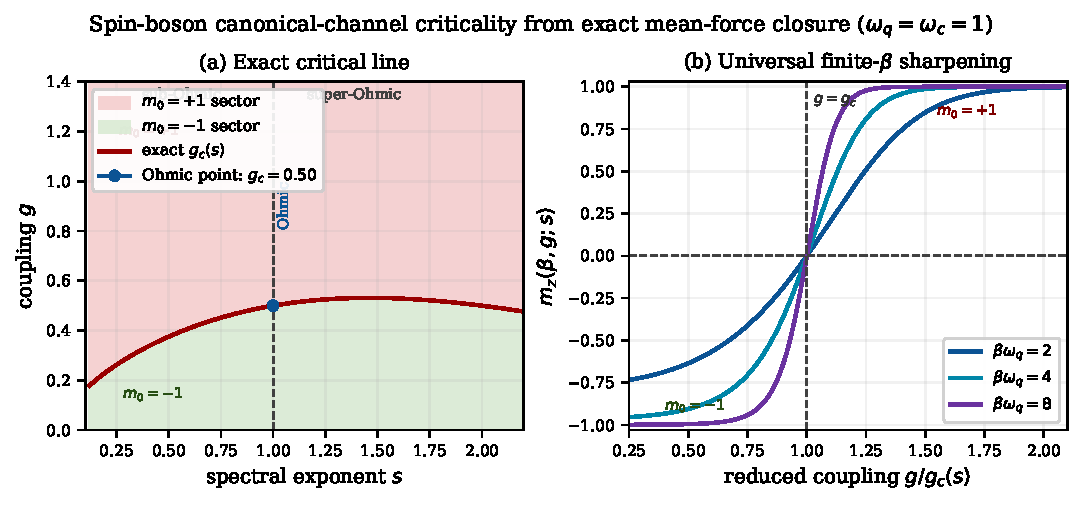
\includegraphics[width=\columnwidth]{../figures/hmf_spin_boson_phase_diagram.pdf}
  \caption{
  Canonical-channel (\(\theta=\pi/2\)) closure threshold by spectral exponent.
  \textbf{(a)} \(g_c(s)=\sqrt{\omega_q/(4\omega_c\Gamma(s))}\) from
  Eq.~\eqref{eq:gc_exact_gamma}.
  \textbf{(b)} Finite-\(\beta\) sharpening in reduced coupling
  \(x=g/g_c(s)\): \(m_z=\tanh[(\beta\omega_q/2)(x^2-1)]\).
  }
  \label{fig:spin_boson_phase_diagram}
\end{figure}

\begin{figure}[tbp]
  \centering
  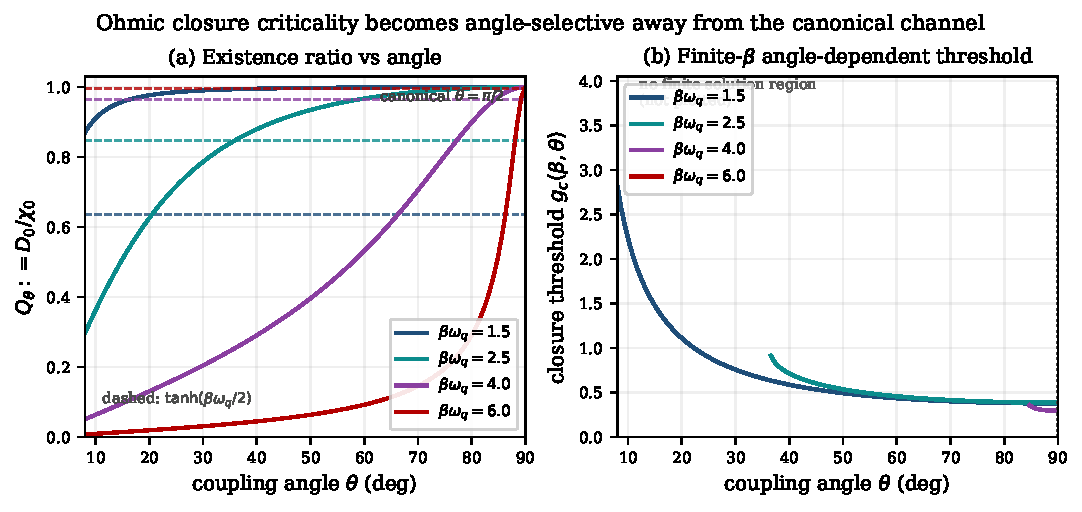
\includegraphics[width=\columnwidth]{../figures/hmf_spin_boson_angle_phase_map.pdf}
  \caption{
  Ohmic (\(s=1\)) angle dependence of the closure threshold.
  \textbf{(a)} Existence ratio \(Q_\theta(\beta)\) versus \(\theta\), compared with
  \(\tanh(\beta\omega_q/2)\) (dashed).
  \textbf{(b)} Finite-\(\beta\) threshold \(g_c(\beta,\theta)\) from
  Eq.~\eqref{eq:gc_angle_finite_beta}; regions with no finite solution are omitted.
  As \(\beta\) increases, the finite-threshold corridor contracts toward \(\theta=\pi/2\).
  }
  \label{fig:spin_boson_angle_phase_map}
\end{figure}

\paragraph{Implementation note.}
Figures~\ref{fig:spin_boson_phase_diagram} and~\ref{fig:spin_boson_angle_phase_map} are generated by
\path{paper_dual_hmf/validation/make_spin_boson_phase_diagram_figure.py} and
\path{paper_dual_hmf/validation/make_spin_boson_angle_phase_figure.py}.

\paragraph{Interpretation and literature scope.}
The \(g_c\) formulas above are closure-level thresholds of the present mean-force construction, with
Eq.~\eqref{eq:gc_exact_gamma} living on the canonical \(\theta=\pi/2\) slice.
They should not be read as a full-universality phase diagram of the spin-boson model for arbitrary
\(\theta\): the established unbiased model phenomenology includes Ohmic KT criticality and no
localization transition in the super-Ohmic case
\cite{leggettDynamicsDissipativeTwostate1987,weissQuantumDissipativeSystems2012}. For sub-Ohmic
dissipation, NRG/QMC and analytic studies report a genuine transition with \(s\)-dependent critical
behavior \cite{bullaQuantumPhaseTransitionSubohmic2003,vojtaQuantumPhaseTransitionsSubohmic2005,winterQuantumPhaseTransitionSubohmic2009,chinGeneralizedPolaronAnsatz2011,bullaNumericalRenormalizationGroup2008}.
The angle-resolved closure map here is therefore a representative-control statement, to be benchmarked
against those nonperturbative universality analyses rather than replacing them.

\subsection{Dual-map analytic entanglement entropy}
\label{subsec:dual_entanglement_entropy}

\paragraph{Closed entropy formula from the Bloch radius.}
For any qubit state with Bloch radius \(r\in[0,1]\), the eigenvalues are
\(\lambda_\pm=(1\pm r)/2\), so the reduced-state von Neumann entropy is
\begin{equation}
  S_Q=-\Tr(\rho_Q\log\rho_Q)
  =-\sum_{\pm}\lambda_\pm\log\lambda_\pm.
\end{equation}
Using the closure relation \(r=|\tanh\chi|\), one obtains the exact analytic form
\begin{equation}
  S_Q(\beta,g,\theta)
  =h_2\!\left(\frac{1+|\tanh\chi(\beta,g,\theta)|}{2}\right),
\end{equation}
where \(h_2(x):=-x\log x-(1-x)\log(1-x)\) and
\(\chi(\beta,g,\theta)=g^2\chi_0(\beta,\theta)\). In the zero-temperature limit, when the joint
state approaches a pure ground state, this equals the system-bath entanglement entropy.

\begin{proposition}[Dual representative entropy map]
\label{prop:dual_entropy_map}
Let \(g^\vee=g_\star^2/g\), so \(\chi^\vee=\chi^{-1}\). Then
\begin{equation}
  S_Q(\beta,g^\vee,\theta)
  =h_2\!\left(\frac{1+|\tanh(\chi^{-1})|}{2}\right).
\end{equation}
Hence the strong-branch entropy at \((\beta,g,\theta)\) is an exact analytic function of the dual
weak coordinate \(\chi^\vee\):
\begin{equation}
  S_Q(\beta,g,\theta)
  =h_2\!\left(\frac{1+|\tanh\!\big((\chi^\vee)^{-1}\big)|}{2}\right).
\end{equation}
\end{proposition}
\begin{proof}
Substitute \(r=|\tanh\chi|\) into the qubit eigenvalue formula and use
\(\chi^\vee=\chi(\beta,g^\vee,\theta)=\chi(\beta,g,\theta)^{-1}\) from
Theorem~\ref{thm:strong_weak_involution}.
\end{proof}

\paragraph{Asymptotic transfer for entropy.}
From the closed form,
\begin{equation}
  S_Q(\chi)=\log 2-\frac{\chi^2}{2}+O(\chi^4),
  \qquad
  \chi\to 0,
\end{equation}
and
\begin{equation}
  S_Q(\chi)=\bigl(1+2\chi\bigr)e^{-2\chi}+O(e^{-4\chi}),
  \qquad
  \chi\to\infty.
\end{equation}
With \(\chi^\vee=\chi^{-1}\), the strong-branch form is equivalently
\begin{equation}
  S_Q=\bigl(1+2/\chi^\vee\bigr)e^{-2/\chi^\vee}+O(e^{-4/\chi^\vee}),
  \qquad
  \chi^\vee\to 0.
\end{equation}

\paragraph{Support from existing analytical and numerical studies.}
The entropy trends encoded above are consistent with prior spin-boson analyses. NRG work found that
for the unbiased Ohmic case the entanglement entropy grows with dissipation and, with bias, develops
a maximum before localization \cite{costiEntanglementQubitEnvironment2003}. Analytical scaling and
field-theory treatments identified universal entanglement structure near the dissipative critical
point \cite{koppUniversalMeasurableEntanglement2007,lehurEntanglementEntropyDecoherence2008}. In
the strong-dissipation regime, variational/multipolaron studies resolved explicit
system-environment entanglement structure compatible with the entropy suppression on localized
branches \cite{beraStabilizingSpinCoherence2014,beraGeneralizedMultipolaron2014}. The dual
representative map presented here adds a closed analytic route that links these branch behaviors by
\(\chi^\vee=\chi^{-1}\).

\begin{figure}[tbp]
  \centering
  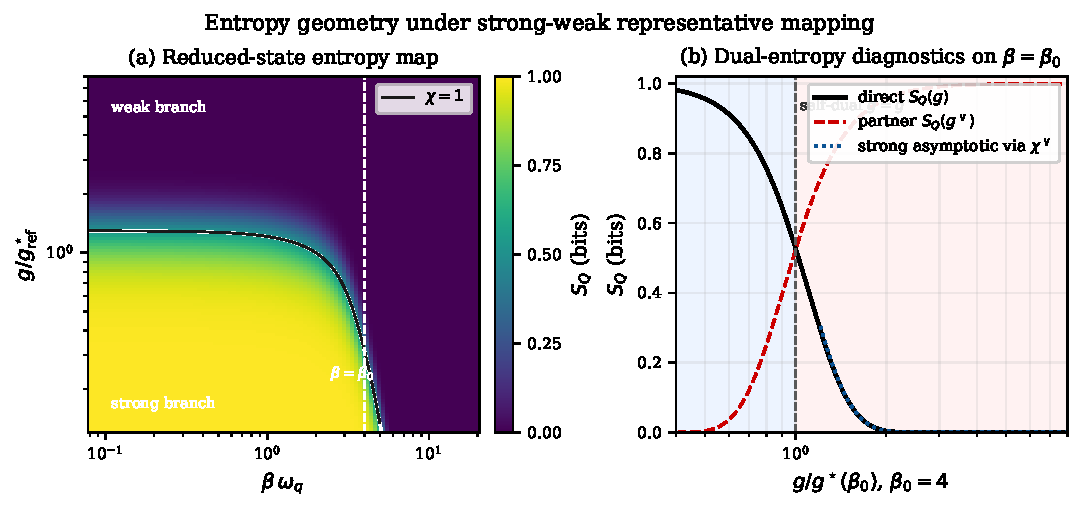
\includegraphics[width=\columnwidth]{../figures/hmf_spin_boson_entropy_duality.pdf}
  \caption{
  Entropy diagnostics from the dual map.
  \textbf{(a)} Reduced-state entropy \(S_Q/\log 2\) across \((\beta,g)\), with the crossover contour
  \(\chi=1\) and the \(\beta=\beta_0\) slice used in panel (b). In the \(\beta\to\infty\) limit
  (pure total ground state), this becomes the system-bath entanglement entropy.
  \textbf{(b)} Coupling sweep at fixed \(\beta_0\): direct entropy \(S_Q(g)\), entropy of the dual
  representative \(S_Q(g^\vee)\) (showing representative non-equality), and strong-branch analytic
  estimate written in the dual weak coordinate \(\chi^\vee=\chi^{-1}\); the vertical marker
  \(g=g^\star(\beta_0)\) indicates the self-dual point.
  }
  \label{fig:spin_boson_entropy_duality}
\end{figure}

\paragraph{Implementation note.}
Figure~\ref{fig:spin_boson_entropy_duality} is generated by
\path{paper_dual_hmf/validation/make_spin_boson_entanglement_duality_figure.py}.
